\begin{minipage}[c]{\textwidth}
\advance\leftskip-2.5cm
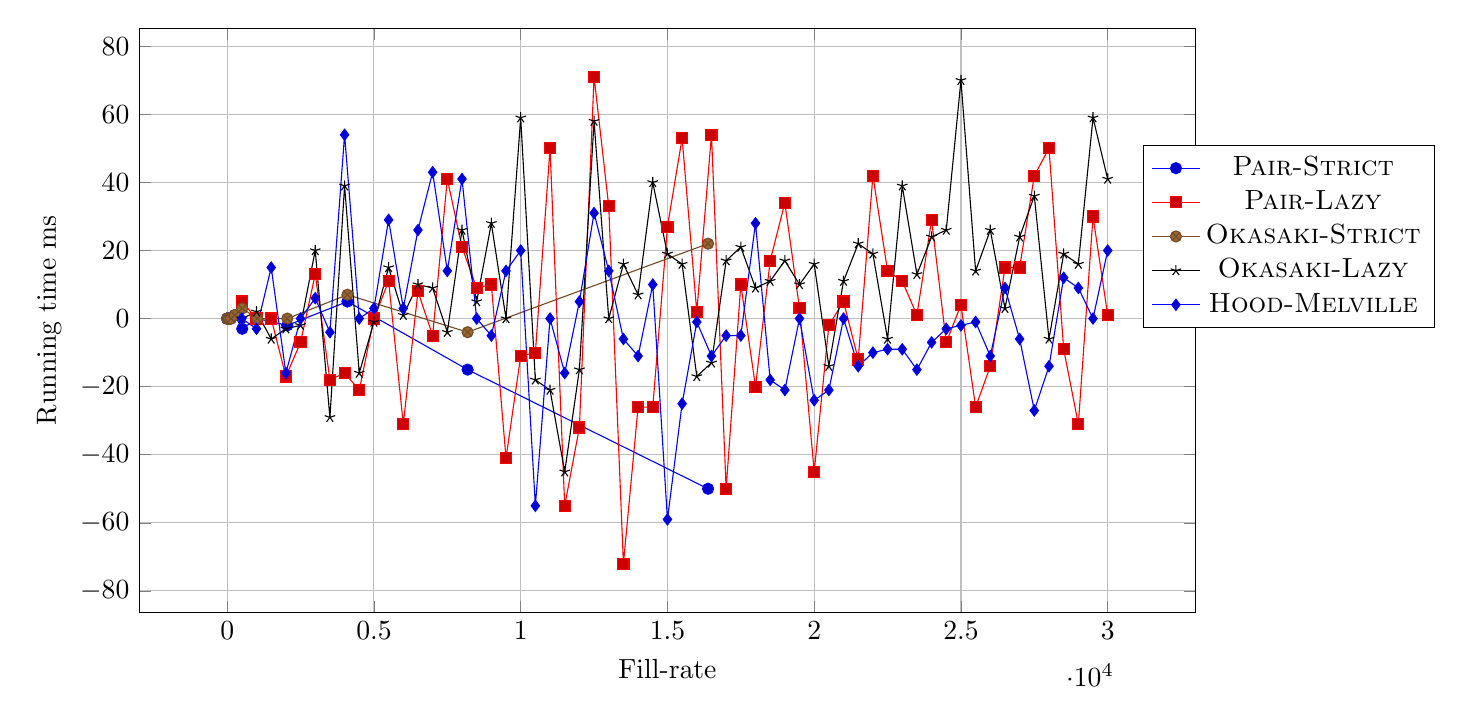
\begin{tikzpicture}
        \begin{axis}[
            xlabel = Fill-rate,
            ylabel = Running time ms,
            height=9cm,
            width=15cm,
            grid=major,
            legend style={
            at={(0.95,0.8)},
            anchor=north west}]            
            legend pos=center west
    	]
    		
  
                \addplot coordinates {
(1,0)
(2,0)
(4,0)
(8,0)
(16,0)
(32,0)
(64,0)
(128,0)
(256,1)
(512,-3)
(1024,0)
(2048,-2)
(4096,5)
(8192,-15)
(16384,-50)

    	};
        
    	\addlegendentry{\textsc{Pair-Strict}}

        \addplot coordinates {
(500,5)
(1000,0)
(1500,0)
(2000,-17)
(2500,-7)
(3000,13)
(3500,-18)
(4000,-16)
(4500,-21)
(5000,0)
(5500,11)
(6000,-31)
(6500,8)
(7000,-5)
(7500,41)
(8000,21)
(8500,9)
(9000,10)
(9500,-41)
(10000,-11)
(10500,-10)
(11000,50)
(11500,-55)
(12000,-32)
(12500,71)
(13000,33)
(13500,-72)
(14000,-26)
(14500,-26)
(15000,27)
(15500,53)
(16000,2)
(16500,54)
(17000,-50)
(17500,10)
(18000,-20)
(18500,17)
(19000,34)
(19500,3)
(20000,-45)
(20500,-2)
(21000,5)
(21500,-12)
(22000,42)
(22500,14)
(23000,11)
(23500,1)
(24000,29)
(24500,-7)
(25000,4)
(25500,-26)
(26000,-14)
(26500,15)
(27000,15)
(27500,42)
(28000,50)
(28500,-9)
(29000,-31)
(29500,30)
(30000,1)

    	};
        
    	\addlegendentry{\textsc{Pair-Lazy}}

        \addplot coordinates {
(1,0)
(2,0)
(4,0)
(8,0)
(16,0)
(32,0)
(64,0)
(128,0)
(256,1)
(512,3)
(1024,0)
(2048,0)
(4096,7)
(8192,-4)
(16384,22)

    	};
        
    	\addlegendentry{\textsc{Okasaki-Strict}}

        \addplot coordinates {
(500,0)
(1000,2)
(1500,-6)
(2000,-3)
(2500,-2)
(3000,20)
(3500,-29)
(4000,39)
(4500,-16)
(5000,-1)
(5500,15)
(6000,1)
(6500,10)
(7000,9)
(7500,-4)
(8000,26)
(8500,5)
(9000,28)
(9500,0)
(10000,59)
(10500,-18)
(11000,-21)
(11500,-45)
(12000,-15)
(12500,58)
(13000,0)
(13500,16)
(14000,7)
(14500,40)
(15000,19)
(15500,16)
(16000,-17)
(16500,-13)
(17000,17)
(17500,21)
(18000,9)
(18500,11)
(19000,17)
(19500,10)
(20000,16)
(20500,-14)
(21000,11)
(21500,22)
(22000,19)
(22500,-6)
(23000,39)
(23500,13)
(24000,24)
(24500,26)
(25000,70)
(25500,14)
(26000,26)
(26500,3)
(27000,24)
(27500,36)
(28000,-6)
(28500,19)
(29000,16)
(29500,59)
(30000,41)

    	};
        
    	\addlegendentry{\textsc{Okasaki-Lazy}}

        \addplot coordinates {
(500,0)
(1000,-3)
(1500,15)
(2000,-16)
(2500,0)
(3000,6)
(3500,-4)
(4000,54)
(4500,0)
(5000,3)
(5500,29)
(6000,3)
(6500,26)
(7000,43)
(7500,14)
(8000,41)
(8500,0)
(9000,-5)
(9500,14)
(10000,20)
(10500,-55)
(11000,0)
(11500,-16)
(12000,5)
(12500,31)
(13000,14)
(13500,-6)
(14000,-11)
(14500,10)
(15000,-59)
(15500,-25)
(16000,-1)
(16500,-11)
(17000,-5)
(17500,-5)
(18000,28)
(18500,-18)
(19000,-21)
(19500,0)
(20000,-24)
(20500,-21)
(21000,0)
(21500,-14)
(22000,-10)
(22500,-9)
(23000,-9)
(23500,-15)
(24000,-7)
(24500,-3)
(25000,-2)
(25500,-1)
(26000,-11)
(26500,9)
(27000,-6)
(27500,-27)
(28000,-14)
(28500,12)
(29000,9)
(29500,0)
(30000,20)

    	};

    	\addlegendentry{\textsc{Hood-Melville}}

        \end{axis}

    \end{tikzpicture}
    \captionof{figure}{TITEL}
    \label{fig:sample_figure}
\end{minipage}